% begin module limit-ex4
\begin{frame}
\begin{example}[Example 4, p. 98]
\begin{columns}[c]
\column{.4\textwidth}
\begin{itemize}
\item  Guess the value of $\lim_{x\rightarrow 0}\sin\frac{\pi}{x}$.
\item<2->  Notice that $\sin\frac{\pi}{x}$ doesn't exist at $0$.  
\item<3->  It does exist at values near $0$.
\item<5->  We guess that the limit is $0$. 
\item<6->  In this case, our guess is \alert<6>{wrong}.
\end{itemize}
\column{.6\textwidth}
\uncover<4->{
\[
\begin{array}{|r|c|r|c|}
\hline
x & f(x) & x & f(x) \\
\hline
1 & \sin \pi = 0 &
\frac{1}{2} & \sin 2\pi = 0 \\
\frac{1}{3} & \sin 3\pi = 0 &
\frac{1}{4} & \sin 4\pi = 0 \\
0.1 & \sin 10\pi = 0 &
0.01 & \sin 100\pi = 0 \\
\hline
\end{array}
\]
}

\uncover<6->{
\ 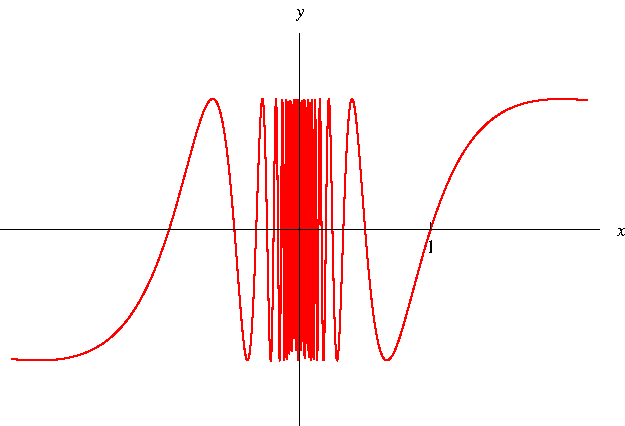
\includegraphics[height=4cm]{limits/pictures/02-01-ex4.pdf}%
}
\end{columns}
\end{example}
\end{frame}
% end module limit-ex4
